% questions.tex —— 2007 年·北京卷·文科 · 题目内容片段（无答案）
% 由 tools/generate_projects.py 依来源总账自 2007/2007_数学真题_北京文_试题.md 生成，勿手改（改源 MD 后重跑）


\gkpart{一、选择题}

\begin{question}
\gkti{1}已知 $\cos\theta\cdot\tan\theta<0$，那么角 $\theta$ 是（　）

\begin{gkopts}(2)
\task （A）第一或第二象限角
\task （B）第二或第三象限角
\task （C）第三或第四象限角
\task （D）第一或第四象限角
\end{gkopts}

\end{question}
\begin{question}
\gkti{2}函数 $f(x)=3^x\ (0<x\leq 2)$ 的反函数的定义域为（　）

\begin{gkopts}(4)
\task （A）$(0,+\infty)$
\task （B）$(1,9]$
\task （C）$(0,1)$
\task （D）$[9,+\infty)$
\end{gkopts}

\end{question}
\begin{question}
\gkti{3}函数 $f(x)=\sin 2x-\cos 2x$ 的最小正周期是（　）

\begin{gkopts}(2)
\task （A）$\dfrac{\pi}{2}$
\task （B）$\pi$
\task （C）$2\pi$
\task （D）$4\pi$
\end{gkopts}

\end{question}
\begin{question}
\gkti{4}椭圆 $\dfrac{x^2}{a^2}+\dfrac{y^2}{b^2}=1\ (a>b>0)$ 的焦点为 $F_1,F_2$，两条准线与 $x$ 轴的交点分别为 $M,N$。若 $|MN|\leq 2|F_1F_2|$，则该椭圆离心率的取值范围是（　）

\begin{gkopts}(2)
\task （A）$\left(0,\dfrac{1}{2}\right]$
\task （B）$\left(0,\dfrac{\sqrt{2}}{2}\right]$
\task （C）$\left[\dfrac{1}{2},1\right)$
\task （D）$\left[\dfrac{\sqrt{2}}{2},1\right)$
\end{gkopts}

\end{question}
\begin{question}
\gkti{5}某城市的汽车牌照号码由 2 个英文字母后接 4 个数字组成，其中 4 个数字互不相同的牌照号码共有（　）

\begin{gkopts}(2)
\task （A）$(C_{26}^{1})^2A_{10}^{4}$ 个
\task （B）$A_{26}^{2}A_{10}^{4}$ 个
\task （C）$(C_{26}^{1})^2 10^4$ 个
\task （D）$A_{26}^{2}10^4$ 个
\end{gkopts}

\end{question}
\begin{question}
\gkti{6}若不等式组

\nopagebreak[4]
\[
\begin{cases}
x-y+5\geq 0,\\
y\geq a,\\
0\leq x\leq 2
\end{cases}
\]

表示的平面区域是一个三角形，则 $a$ 的取值范围是（　）

\begin{gkopts}(2)
\task （A）$a<5$
\task （B）$a\geq 7$
\task （C）$5\leq a<7$
\task （D）$a<5$ 或 $a\geq 7$
\end{gkopts}

\end{question}
\begin{question}
\gkti{7}平面 $\alpha\parallel$ 平面 $\beta$ 的一个充分条件是（　）

（A）存在一条直线 $a$，$a\parallel\alpha$，$a\parallel\beta$

（B）存在一条直线 $a$，$a\subset\alpha$，$a\parallel\beta$

（C）存在两条平行直线 $a,b$，$a\subset\alpha$，$b\subset\beta$，$a\parallel\beta$，$b\parallel\alpha$

（D）存在两条异面直线 $a,b$，$a\subset\alpha$，$b\subset\beta$，$a\parallel\beta$，$b\parallel\alpha$

\end{question}
\begin{question}
\gkti{8}对于函数① $f(x)=|x+2|$，② $f(x)=(x-2)^2$，③ $f(x)=\cos(x-2)$，判断如下两个命题的真假：

命题甲：$f(x+2)$ 是偶函数；

命题乙：$f(x)$ 在 $(-\infty,2)$ 上是减函数，在 $(2,+\infty)$ 上是增函数；

能使命题甲、乙均为真的所有函数的序号是（　）

\begin{gkopts}(4)
\task （A）①②
\task （B）①③
\task （C）②
\task （D）③
\end{gkopts}

\end{question}
\gkpart{二、填空题}

\begin{question}
\gkti{9}$f'(x)$ 是 $f(x)=\dfrac{1}{3}x^3+2x+1$ 的导函数，则 $f'(-1)$ 的值是\gkblank{}。

\end{question}
\begin{question}
\gkti{10}若数列 $\{a_n\}$ 的前 $n$ 项和 $S_n=n^2-10n\ (n=1,2,3,\ldots)$，则此数列的通项公式为\gkblank{}。

\end{question}
\begin{question}
\gkti{11}已知向量 $\boldsymbol a=(2,4)$，$\boldsymbol b=(1,1)$。若向量 $\boldsymbol b\perp(\boldsymbol a+\lambda\boldsymbol b)$，则实数 $\lambda$ 的值是\gkblank{}。

\end{question}
\begin{question}
\gkti{12}在 $\triangle ABC$ 中，若 $\tan A=\dfrac{1}{3}$，$C=150^\circ$，$BC=1$，则 $AB=$\gkblank{}。

\Needspace{0.4\textheight}
\end{question}
\begin{question}
\gkti{13}2002 年在北京召开的国际数学家大会，会标是以我国古代数学家赵爽的弦图为基础设计的。弦图是由四个全等直角三角形与一个小正方形拼成的一个大正方形（如图）。如果小正方形的面积为 1，大正方形的面积为 25，直角三角形中较小的锐角为 $\theta$，那么 $\cos 2\theta$ 的值等于\gkblank{}。
\nopagebreak[4]
\begin{center}% 依据固定候选 PDF 第 1 页重绘；source_id=src-71817304e261efb7deaf51c2a5f400421a95ac91a90313d8f558bee701a624f9
% PDF SHA-256: e5356797259eb22cc2b4f23019ad7ab044f282bdfc2a65df94dbbdcc502cfff5
% 按源图保留外正方形、中心正方形及四个全等直角三角形；源图没有角度标注。
\begin{center}
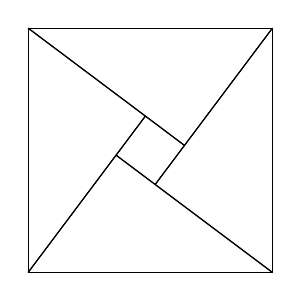
\begin{tikzpicture}[scale=0.62,line join=round,line cap=round]
  \coordinate (A) at (0,0);
  \coordinate (B) at (5,0);
  \coordinate (C) at (5,5);
  \coordinate (D) at (0,5);
  \coordinate (P) at (1.8,2.4);
  \coordinate (Q) at (2.6,1.8);
  \coordinate (R) at (3.2,2.6);
  \coordinate (S) at (2.4,3.2);
  \draw (A)--(B)--(C)--(D)--cycle;
  \draw (A)--(P)--(B);
  \draw (B)--(Q)--(C);
  \draw (C)--(R)--(D);
  \draw (D)--(S)--(A);
  \draw (P)--(Q)--(R)--(S)--cycle;
\end{tikzpicture}
\end{center}
\end{center}
\nopagebreak[4]
\end{question}
\begin{question}
\gkti{14}已知函数 $f(x)$，$g(x)$ 分别由下表给出：

\begin{center}
\begin{tabular}{lrrr}
\toprule
$x$ & 1 & 2 & 3 \\
\midrule
$f(x)$ & 2 & 1 & 1 \\
\bottomrule
\end{tabular}
\end{center}

\begin{center}
\begin{tabular}{lrrr}
\toprule
$x$ & 1 & 2 & 3 \\
\midrule
$g(x)$ & 3 & 2 & 1 \\
\bottomrule
\end{tabular}
\end{center}

则 $f[g(1)]$ 的值为\gkblank{}；当 $g[f(x)]=2$ 时，$x=$\gkblank{}。

\end{question}
\begin{question}
\gkti{15}记关于 $x$ 的不等式 $\dfrac{x-a}{x+1}<0$ 的解集为 $P$，不等式 $|x-1|\leq 1$ 的解集为 $Q$。

(1) 若 $a=3$，求 $P$；

(2) 若 $Q\subseteq P$，求正数 $a$ 的取值范围。

\end{question}
\begin{question}
\gkti{16}数列 $\{a_n\}$ 中，$a_1=2$，$a_{n+1}=a_n+cn$（$c$ 是常数，$n=1,2,3,\ldots$），且 $a_1,a_2,a_3$ 成公比不为 1 的等比数列。

(1) 求 $c$ 的值；

(2) 求 $\{a_n\}$ 的通项公式。

\end{question}
\gkpart{三、解答题}

\Needspace{0.4\textheight}
\begin{question}
\gkti{17}如图，在 $\mathrm{Rt}\triangle AOB$ 中，$\angle OAB=\dfrac{\pi}{6}$，斜边 $AB=4$。$\mathrm{Rt}\triangle AOC$ 可以通过 $\mathrm{Rt}\triangle AOB$ 以直线 $AO$ 为轴旋转得到，且二面角 $B-AO-C$ 是直二面角。$D$ 是 $AB$ 的中点。

(1) 求证：平面 $COD\perp$ 平面 $AOB$；

(2) 求异面直线 $AO$ 与 $CD$ 所成角的大小。
\nopagebreak[4]
\begin{center}% 依据固定候选 PDF 第 1 页重绘；source_id=src-71817304e261efb7deaf51c2a5f400421a95ac91a90313d8f558bee701a624f9
% PDF SHA-256: e5356797259eb22cc2b4f23019ad7ab044f282bdfc2a65df94dbbdcc502cfff5
% 保留原图边界、D 位于 AB、CD 实线以及 AO、OB、OC、OD 虚线关系；示意图不按比例。
\begin{center}
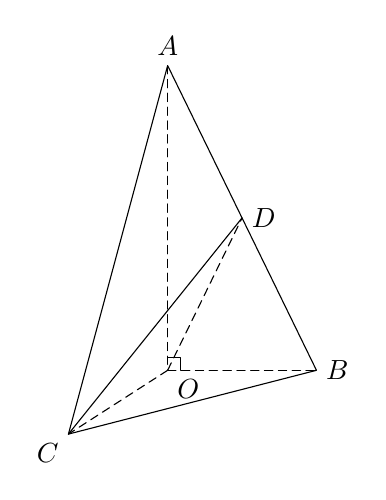
\begin{tikzpicture}[x=0.9cm,y=0.9cm,line join=round,line cap=round]
  \coordinate (A) at (0,4.3);
  \coordinate (O) at (0,0);
  \coordinate (B) at (2.1,0);
  \coordinate (C) at (-1.4,-0.9);
  \coordinate (D) at (1.05,2.15);
  \draw (A)--(C)--(B)--cycle;
  \draw (C)--(D);
  \draw[densely dashed] (A)--(O);
  \draw[densely dashed] (O)--(B);
  \draw[densely dashed] (O)--(C);
  \draw[densely dashed] (O)--(D);
  \draw (0.18,0)--(0.18,0.18)--(0,0.18);
  \node[above] at (A) {$A$};
  \node[right] at (B) {$B$};
  \node[below left] at (C) {$C$};
  \node[below right] at (O) {$O$};
  \node[right] at (D) {$D$};
\end{tikzpicture}
\end{center}
\end{center}
\nopagebreak[4]
\end{question}
\begin{question}
\gkti{18}某条公共汽车线路沿线共有 11 个车站（包括起点站和终点站）。在起点站开出的一辆公共汽车上有 6 位乘客，假设每位乘客在起点站之外的各个车站下车是等可能的。求：

(1) 这 6 位乘客在互不相同的车站下车的概率；

(2) 这 6 位乘客中恰有 3 人在终点站下车的概率。

\Needspace{0.4\textheight}
\end{question}
\begin{question}
\gkti{19}如图，矩形 $ABCD$ 的两条对角线相交于点 $M(2,0)$，$AB$ 边所在直线的方程为 $x-3y-6=0$，点 $T(-1,1)$ 在 $AD$ 边所在直线上。

(1) 求 $AD$ 边所在直线的方程；

(2) 求矩形 $ABCD$ 外接圆的方程；

(3) 若动圆 $P$ 过点 $N(-2,0)$，且与矩形 $ABCD$ 的外接圆外切，求动圆 $P$ 的圆心的轨迹方程。
\nopagebreak[4]
\begin{center}% 依据固定候选 PDF 第 2 页重绘；source_id=src-71817304e261efb7deaf51c2a5f400421a95ac91a90313d8f558bee701a624f9
% PDF SHA-256: e5356797259eb22cc2b4f23019ad7ab044f282bdfc2a65df94dbbdcc502cfff5
% 坐标按题设精确重建：A(0,-2)、B(24/5,-2/5)、C(4,2)、D(-4/5,2/5)，M(2,0)、T(-1,1)。
\begin{center}
\begin{tikzpicture}[x=0.78cm,y=0.78cm,line join=round,line cap=round]
  \coordinate (A) at (0,-2);
  \coordinate (B) at (4.8,-0.4);
  \coordinate (C) at (4,2);
  \coordinate (D) at (-0.8,0.4);
  \coordinate (M) at (2,0);
  \coordinate (N) at (-2,0);
  \coordinate (O) at (0,0);
  \coordinate (T) at (-1,1);
  \draw[->] (-2.8,0)--(6.15,0) node[below] {$x$};
  \draw[->] (0,-3.3)--(0,2.8) node[above] {$y$};
  \draw (A)--(B)--(C)--(D)--cycle;
  \draw (-1.4,2.2)--(0.5,-3.5);
  \fill (N) circle (1.1pt);
  \fill (M) circle (1.1pt);
  \fill (T) circle (1.1pt);
  \node[above left] at (N) {$N$};
  \node[above] at (M) {$M$};
  \node[below right] at (O) {$O$};
  \node[above left] at (T) {$T$};
  \node[below left] at (A) {$A$};
  \node[below right] at (B) {$B$};
  \node[above right] at (C) {$C$};
  \node[above left] at (D) {$D$};
\end{tikzpicture}
\end{center}
\end{center}
\nopagebreak[4]
\end{question}
\begin{question}
\gkti{20}已知函数 $y=kx$ 与 $y=x^2+2\ (x\geq 0)$ 的图象相交于 $A(x_1,y_1)$，$B(x_2,y_2)$。$l_1,l_2$ 分别是 $y=x^2+2\ (x\geq 0)$ 的图象在 $A,B$ 两点的切线，$M,N$ 分别是 $l_1,l_2$ 与 $x$ 轴的交点。

(1) 求 $k$ 的取值范围；

(2) 设 $t$ 为点 $M$ 的横坐标，当 $x_1<x_2$ 时，写出 $t$ 以 $x_1$ 为自变量的函数式，并求其定义域和值域；

(3) 试比较 $|OM|$ 与 $|ON|$ 的大小，并说明理由（$O$ 是坐标原点）。

\begin{gktip}
\textbf{来源说明}：题面据固定候选 PDF 逐题转录；该文件仅含题面。发布者、版本、复制链与官方身份未核。
\end{gktip}

\end{question}